\documentclass[12pt,oneside]{article}
\usepackage{light}
\usepackage{multicol}
\usepackage{pifont} % for the star
\usepackage{palatino}
\usepackage{mathpazo}
\usepackage{verbatim}

\newcommand{\mfigure}[3]{\bigskip\centerline{\resizebox{#1}{#2}{\includegraphics{#3}}}\bigskip}
\newcommand{\hint}[1]{({\it Hint: #1})}
\newcommand{\brule}[1]{\underline{\hspace{#1}}}
\newcommand{\ang}[1]{\left< #1 \right>}
\newcommand{\beats}{\rightarrow}


\newenvironment{falseproof}
{\begin{proof}[False proof]}
{\end{proof}}

%\showsolutions
\hidesolutions

\begin{document}
\generic{Midterm}{October 27, 2010}

\instatements{
\vspace{12pt}
\textbf{Name:} \rule{5in}{0.5pt}

\textbf{Circle the name of your recitation instructor}:

\begin{center}
\begin{tabular}{llllll}
David & Darren & Martyna & Nick & Oscar & Stav 
\end{tabular}
\end{center}

\begin{itemize}

\item This quiz is \textbf{closed book}, but you may have one $8.5
\times 11$'' sheet with notes in your own handwriting on both sides.

\item Calculators are not allowed.

\item You may assume all of the results presented in class.

\item Please show your work.  Partial credit cannot be given for a wrong
answer if your work isn't shown.

\item Write your solutions in the space provided.  If you
need more space, write on the back of the sheet containing the
problem.  Please keep your entire answer to a problem on that
problem's page.

\item Be neat and write legibly.  You will be graded not only on the
correctness of your answers, but also on the clarity with which you
express them.

\item If you get stuck on a problem, move on to others. The problems 
are not arranged in order of difficulty.

\item The exam ends at 9:30 PM.

\end{itemize}

\vspace{0.25in}

\begin{center}
{\large
\begin{tabular}{|c|c|c|c|}
\hline
Problem & Points & Grade & Grader \\ \hline \hline
1 & 10 & & \\ \hline
2 & 15 & & \\ \hline
3 & 20 & & \\ \hline
4 & 15 & & \\ \hline
5 & 18 & & \\ \hline
6 & 20 & & \\ \hline
7 & 10 & & \\ \hline
8 & 12 & & \\ \hline
Total & 120 & & \\ \hline
\end{tabular}
}
\end{center}
}
\instatements{\newpage}



\begin{problem}{10}

Consider these two propositions:
$$\texttt{P: } (A \wedge B) \implies C$$
$$\texttt{Q: } (\neg C \implies \neg A) \vee (\neg C \implies \neg B)$$ 

Use the truth table below to show whether $P$ and $Q$ are equivalent, $P \implies Q$, $Q \implies P$, or none of the above.

\[
\begin{array}{|c|c|c|c|c|}
\hline
A & B & C & (A \vee B) \implies C & (\neg C \implies \neg A) \vee (\neg C \implies \neg B) \\ \hline
& & & & \\ \hline
& & & & \\ \hline
& & & & \\ \hline
& & & & \\ \hline
& & & & \\ \hline
& & & & \\ \hline
& & & & \\ \hline
& & & & \\ \hline
\end{array}
\]

\solution{

\[
\begin{array}{|c|c|c|c|c|}
\hline
A & B & C & (A \vee B) \implies C & (\neg C \implies \neg A) \vee (\neg C \implies \neg B) \\ \hline
T & T & T & T & T \\ \hline
T & T & F & F & F \\ \hline
T & F & T & T & T \\ \hline
T & F & F & F & T \\ \hline
F & T & T & T & T \\ \hline
F & T & F & F & T \\ \hline
F & F & T & T & T \\ \hline
F & F & F & T & T \\ \hline
\end{array}
\]

Observe from the last two columns of the table that $P \implies Q$ is always true, but $Q \implies P$ is not always true (e.g. line $4$).  Thus $P$ and $Q$ are not equivalent but $P \implies Q$. 

}

\end{problem}

\newpage


%%%%%%%%%%%%%%%%%%%%%%%%%%%%%%%%%%%%%%%%%%%%%%%%%%%%%%%%%%%%%%%%%%%%%%%%%%%%%%%%%%%%%%%%%%%%%%%%%%%%%%%% Strong Induction
\begin{problem}{15}

Let $G_0=1$, $G_1=2$, $G_2=4$, and define
\begin{equation}\label{Pn}
G_n =  G_{n-1} +2G_{n-2} + G_{n-3}
\end{equation}
for $n \geq 3$.  Show by induction that $G_n\leq 3^n$ for all $n \geq
0$.

\solution{

The proof is by strong induction with hypothesis $P(n) := G_n\leq 3^n$.

\begin{proof}
\textbf{Base Cases}

\textbf{$n=0$:} $G_0 = 1 = 3^0$.

\textbf{$n=1$:} $G_1 = 2 < 3 = 3^1$.

\textbf{$n=2$:} $G_2 =f 4 < 9 < 3^2$.

\textbf{Inductive Step}:
Assume $n \geq 2$ and $P(k)$ for all $k$ such that $0 \leq k \leq n$.
\begin{align*}
G_{n+1}
& = G_n +2G_{n-1} + G_{n-2} & \text{by~\eqref{Pn}}\\
& \leq 3^n + (2)3^{n-1} + 3^{n-2} & \text{by induction hypothesis}\\
& = 3^{n-2} [3^2 + (2)3 + 1]\\
& = 3^{n-2} [(3 + 1)^2]\\
& = 3^{n-2} 4^2\\
& = 3^{n-2} 16\\
& < 3^{n-2} 27\\
& = 3^{n-2} 3^3\\
& = 3^{n+1}
\end{align*}
\end{proof}
}
\end{problem}


\newpage

%%%%%%%%%%%%%%%%%%%%%%%%%%%%%%%%%%%%%%%%%%%%%%%%%%%%%%%%%%%%%%%%%%%%%%%%%%%%%%%%%%%%%%%%%%%%%%%%%%%%%%% squares and circles game
\begin{problem}{20}
%Taken from: http://www.cut-the-knot.org/ctk/invariant.shtml

In the game of Squares and Circles, the players (you and your computer) start with a sequence of shapes: some circles and some squares. On each move a player chooses any two shapes from the sequence. These two are replaced with a single one according to the following rule:

Identical shapes are replaced with a square. Different shapes are replaced with a circle.

At the end of the game, when only one shape remains, you are a winner if the remaining shape is a circle. Otherwise, your computer wins. 

\bparts

\ppart{5}
Prove that the game will end.

\solution[\vspace{2in}]{ Todo.}

\ppart{15}
Prove that you will win if the number of circles initially is odd. Hint: Use an invariant about the number of circles.
 
\solution{ Todo.}

\eparts

\end{problem}

%%%%%%%%%%%%%%%%%%%%%%%%%%%%%%%%%%%%%%%%%%%%%%%%%%%%%%%%%%%%%%%%%%%%%%%%%%%%%%%%%%%%%%%%%%%%%%%%%%%%%%%%%%%%%%%%%%%%%%%%%%%%%%%% pulverizer / finding inverses
\newcommand{\card}[1]{\left|#1\right|}

%number theory

\newpage

\begin{problem}{15}
\bparts
\ppart{8}
Find a number $x \in \{0, 1, \ldots, 112\}$ such that $18x \equiv 1 \pmod{113}$.

\solution[\vspace{4in}]{

We can do this using the pulverizer.  Specifically, if we find a pair $(s, t)$ such that $18s + 113t = 1$, then we know that $18s \equiv 1 \pmod{113}$.
\[
\begin{array}{ccccrcl}
x & \quad & y & \quad & \rem(x,y) & = & x - q \cdot y \\ \hline
113 && 18 && 5  & = &   113 - 6 \cdot 18 \\
18 && 5 && 3   & = &   18 - 3 \cdot 5 \\
&&&&            & = &   18 - 3 \cdot (113 - 6 \cdot 18) \\
&&&&            & = &   -1 \cdot 113 + 19 \cdot 18 \\
5 && 3  && 2   & = &   5 - 3 \\
&&&&						& = & (113 - 6 \cdot 18) - (-1 \cdot 113 + 19 \cdot 18) \\
&&&&            & = &   (2 \cdot 113 - 25 \cdot 18) \\
3 && 2 && 1 & = & 3 - 2 \\
&&&&            & = & (-1 \cdot 113 + 19 \cdot 18 ) - (2 \cdot 113 - 25 \cdot 18) \\
&&&&            & = &   \fbox{$-3 \cdot 113 + 44 \cdot 18$} \\
\end{array}
\]
So the multiplicative inverse of $18$ modulo $113$ is $44$.
}

\ppart{7}
Find a number $y \in \{0, 1, \ldots, 112\}$ such that $18^{112111} \equiv y \pmod{113}$
\hint{What power of $18$ is $x$ congruent to modulo $113$?}
\solution{By Fermat's Theorem, since $113$ is prime and $113$ and $18$ are relatively prime, it must be that
\[18\cdot 18^{111} \equiv 18^{113-1} \equiv 1 \pmod {113},\]
so $x \equiv 111 \pmod {113}$.
As a result,
\[18^{112111} \equiv 18^{112\cdot 1000 + 111} \equiv {18^{112}}^1000 \cdot 18^{111} \equiv 1^{1000} \cdot x \equiv x \equiv 44 \pmod {113},\]
so the answer is $44$.
}

\eparts
\end{problem}

\newpage

%%%%%%%%%%%%%%%%%%%%%%%%%%%%%%%%%%%%%%%%%%%%%%%%%%%%%%%%%%%%%%%%%%%%%%%%%%%%%%%%%%%%%%%%%%%%%%%%%%%%%%%%%%%%%% concrete graph problem

\newpage

\begin{problem}{18}

Consider the simple graph $G$ given in figure $X$.

\begin{figure}[h]
\caption{Simple graph G}
\begin{center}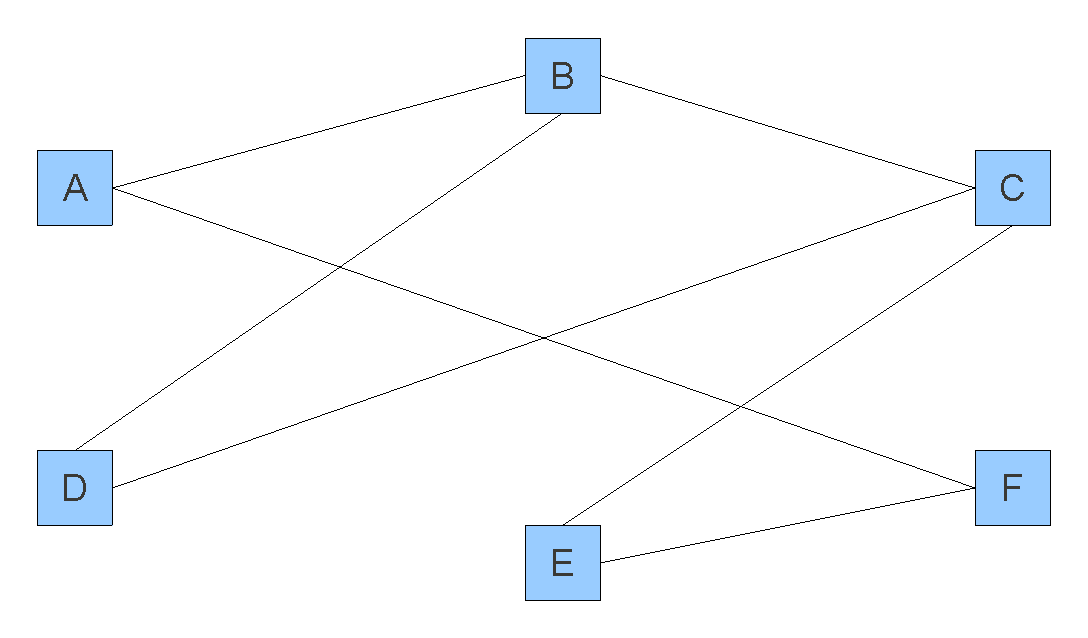
\includegraphics[width=12cm]{unweightedGraph.pdf}\end{center}
\end{figure}

\bparts

\ppart{3}
Give the diameter of $G$.
\solution[\vspace{0.5in}]{
Recall that the diameter is the maximum of all shortest path lengths between pairs of vertices.  Note that the shortest path between $D$ and $F$ is $3$, and all other pairs of non-adjacent vertices share a neighbor.
}

\ppart{3}
Give a longest path on $G$.
\solution[\vspace{0.5in}]{
One possible solution is $(A, F, E, C, D, B)$.  This path has length equal to $|V|$ so it's a longest path.  (There are many possible solutions; just check that the solution is a path of length $6$.)
}

\ppart{3}
Give a coloring on $G$ and show that it uses the smallest possible number of colors.
\solution[\vspace{0.7in}]{
One possible $3$-coloring is: $A$, $D$, $E$ red; $B$, $F$ green; $C$ blue.  Because there exists an odd-length cycle (e.g. $B$, $D$, $C$), no $2$-coloring exists.  Therefore the given coloring uses the least possible number of colors. 
}

\ppart{3}
Does $G$ have an Eulerian cycle?  Justify your answer.
\solution[\vspace{1in}]{No.  This follows from the fact that there exist vertices with odd degree; e.g. $B$.}

\eparts

\newpage
Now consider graph $H$, which is like $G$ but with weighted edges, in figure $Y$:

\begin{figure}[h]
\caption{Weighted graph H}
\begin{center}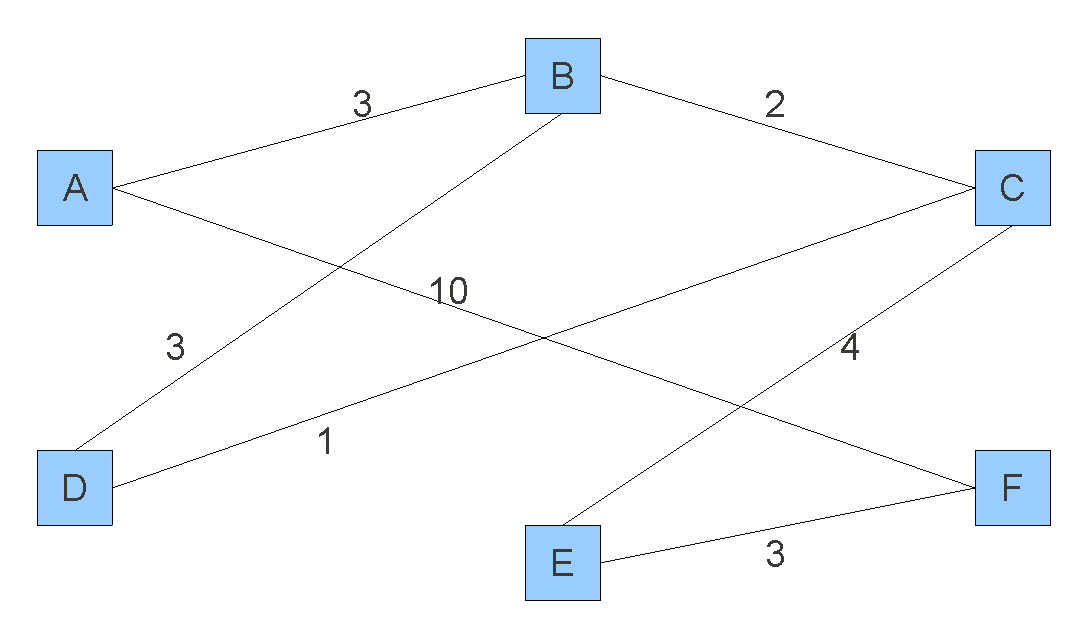
\includegraphics[width=12cm]{weightedGraph.pdf}\end{center}
\end{figure}

\bparts

\ppart{3}
Draw a minimum spanning tree on $H$.
\solution[\vspace{0.5in}]{
\begin{figure}[h]
\caption{MST on graph H}
\begin{center}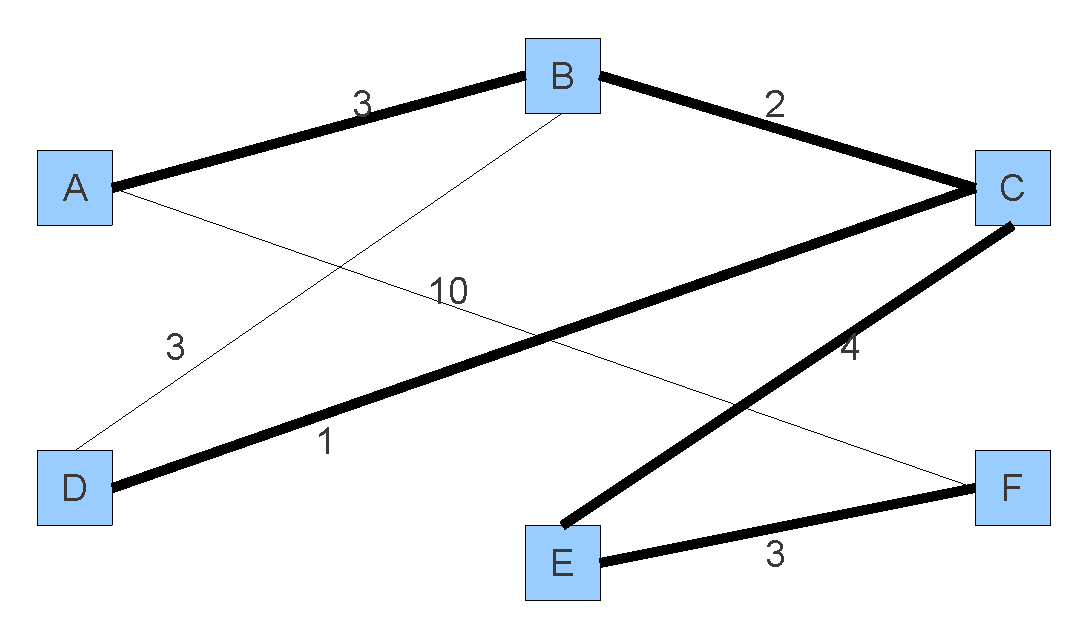
\includegraphics[width=12cm]{mstGraph.pdf}\end{center}
\end{figure}

The darkened edges in figure $Z$ represent the edges in an MST on $H$.  In fact this is the only possible $MST$, as a run through the greedy algorithm confirms.
}

\ppart{3}
Give a list of edges reflecting the order in which a greedy algorithm would choose edges when finding an MST on $H$.
\solution[\vspace{1in}]{
There are two possible responses: $((C,D), (B,C), (A,B), (E,F), (C,E))$ and $((C,D), (B,C), (E,F), (A,B), (C,E))$.  No other order is possible using the greedy algorithm presented in this class.
}

\eparts
\end{problem}

\newpage

%%%%%%%%%%%%%%%%%%%%%%%%%%%%%%%%%%%%%%%%%%%%%%%%%%%%%%%%%%%%%%%%%%%%%%%%%%%%%%%%%%%%%%%%%%%%%%%%%%%%%%%%%%%%%%%% graph induction on edges
\newpage

\begin{problem}{20}
Let G be a graph with $n$ vertices, $m$ edges and $k$ components. Prove that $G$ contains at least $m + k - n  = c$ cycles. (Hint: Prove this by induction on the number of edges, $m$)

\solution{
The proof is by induction on m with hypothesis P(n):= If G is a graph with $n$ vertices, $m$ edges and $k$ components, then $G$ contains at least  $m + k -n = c$ cycles

\begin{proof}

\textbf{Base Case}
$m=0$: Let G be any graph with 0 edges and $n$ vertices. Then since there are no edges,  each vertex is its own connected component, hence there are $k=n$ connected components. Since there are no edges there are also no cycles so $c=0$. Lastly we note that $m+k-n=n+0-n=0$, and hence our base case. 

\textbf{Inductive Step}
Assume that P(m) holds, that is any graph with $m$ edges, $n$ vertices, and $k$ components has at least $m+k-n$ cycles. We must show that P(m+1) holds.

Consider an arbitrary graph $G$ with $m+1$ edges, $n$ vertices, and $k$ components. Suppose we remove an arbitrary edge, $e$, from $G$ to obtain $G'$. This edge, $e$, was either in a cycle in G or not:

\textit{Case 1:} $e$ is part of a cycle in $G$

If $e$ is in a cycle in $G$ then removing it removes at least one cycle. Furthermore, removing $e$ does not disconnect the graph so the number of components remains the same. So $G'$ has $m$ edges, $n$ vertices, and $k$ components, which by the inductive hypothesis tells us it has at least $m+k-n$ cycles. But $G$ has at least one more cycle than $G'$ (since $e$ is part of a cycle). So $G$ has at least $m+k-n +1$, or $(m+1)+k-n$ cycles, as desired.

\textit{Case 2:} $e$ is not part of a cycle in G
If $e$ is not part of a cycle removing it disconnects the graph of G, so the number of components in $G'$ is $k+1$. So, $G'$ contains $m$ edges, $n$ vertices, and $k+1$ components, so by the inductive hypothesis it contains at least $m+(k+1)-n$ cycles. Now since $e$ was not part of a cycle, $G$ and $G'$ have the same number of cycles. So $G$ also has at least$m+(k+1)-n$ cycles. Rearranging we get that $G$ has at least $(m+1)+k-n$ cycles as desired.

\end{proof}
}

\end{problem}

\newpage

%%%%%%%%%%%%%%%%%%%%%%%%%%%%%%%%%%%%%%%%%%%%%%%%%%%%%%%%%%%%%%%%%%%%%%%%%%%%%%%%%%%%%%%%%%%%%%%%%%%%%%%%%%%%%%%%%%%%%%%%%%%%%%%%%%% bounding sums

\begin{problem}{10}
Use integration to find upper and lower bounds that differ by at most 1 for the following sum.
%
\[
\sum_{i=1}^{\infty} \frac{1}{i^4}
\]

\end{problem}


\newpage

%%O notation problem (Oscar) %%%%%%
\begin{problem}{12}
Give a proof of the following propositions.

\bparts

\ppart{3}
$x$ is $O\left( x\ln{x} \right)$
\solution[\vspace{1.5in}]{//TODO}
\ppart{3}
$x/ \ln{x}$  is $o  \left( x \right)$
\solution[\vspace{1.5in}]{//TODO}
\ppart{3}
$x^{n+1}$ is $\Omega \left( x^n \right)$
\solution[\vspace{1.5in}]{//TODO}
\ppart{3}
$n!$ is $\omega \left( n^n \right)$
\solution[\vspace{1.5in}]{//TODO}

\eparts
\end{problem}

\end{document}
